Classic magnetism question.

\begin{parts}
	\part
	\begin{figure}[H]
		\centering
		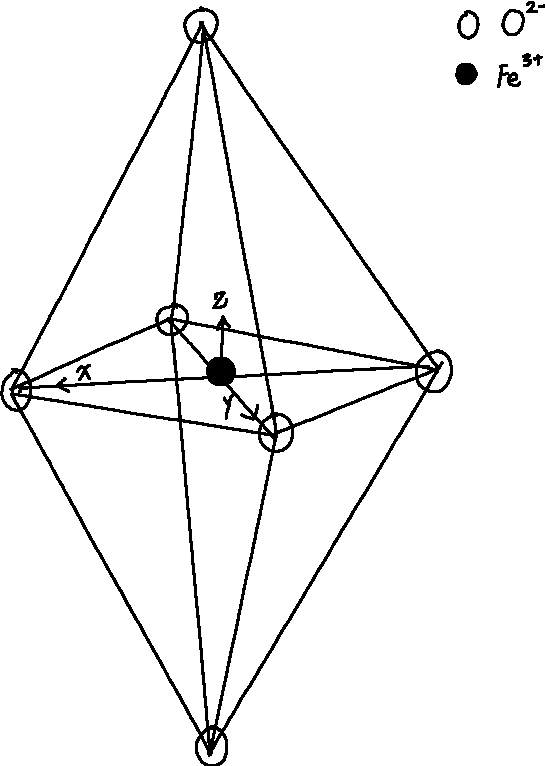
\includegraphics[width=.5\linewidth]{q5-octahedral}
	\end{figure}
	As shown in the diagram above, as the \ion{O}{$2-$} ions are located along the principal axes, the $3d$ orbitals of the central Fe ion along $x$, $y$, $z$ have greater overlap with the \ion{O}{$2-$} orbitals, thereby experiencing greater Coulomb repulsion $\Rightarrow$ higher energy, this splitting also causes the effective orbital angular momentum to vanish, this is called \textit{orbital quenching}.
	Strength of the field can alter the magnetic ground state as above.
	
	At high pressure when the crystal is compressed, the crystal field effectively increases and lead to the transition above, the slight mismatch between the low field $\mu_\textnormal{eff}$ is due to the strength of crystal field not being strong enough to fully quench $L$.
	
	\part
	\begin{figure}[H]
		\centering
		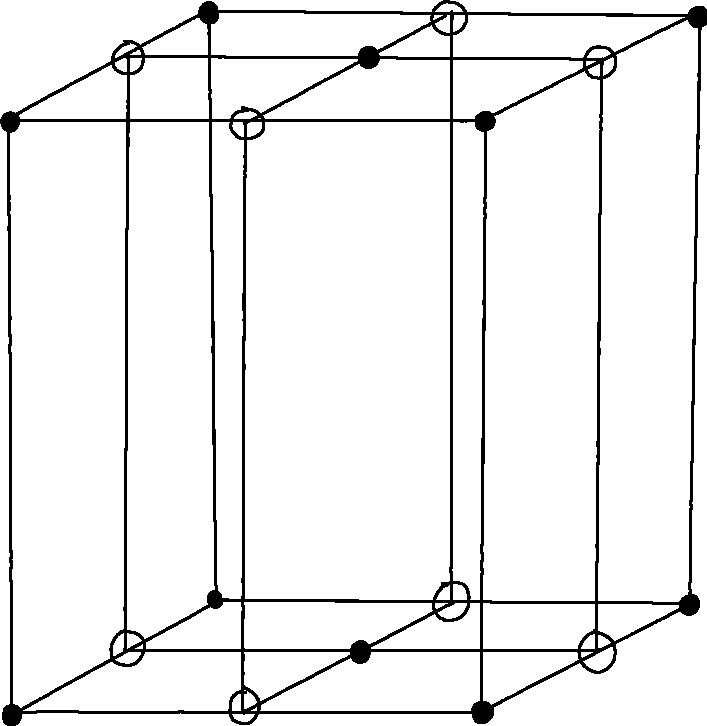
\includegraphics[width=.5\linewidth]{q5-magnetic-lattice}
	\end{figure}
	Note that the magnetic UC has dimensions $2a \times 2a \times c$ with c-centering.
	The sublattices are located $a\hat{\mathbf{x}}$ from one another.
	
	Thus the structure factor is:
	\begin{equation*}
		S = f\sbracket{1 + \mathrm{e}^{2\pi i \rbracket{ha/2a + ka/2a + 0}}} - f\mathrm{e}^{2\pi i \rbracket{ha/2a}} \sbracket{1 + \mathrm{e}^{2\pi i \rbracket{ha/2a + ka/2a + 0}}}
	\end{equation*}
	So for $S$ to vanish, $h+k$ must be odd.
	
	Miller indices with the smallest $k$'s: (1,0,0) and (0,1,0).
	
	\part Nearest-neighbour Heisenberg: $\mathcal{H} = \sum_{i,j} -J_1 / 2 \, \mathbf{S}_i \cdot \mathbf{S}_j + J_2 / 2 \rbracket{\mathbf{S}_i}^2$.
	
	$B_\textnormal{mf}$ is the molecular mean field -- this is the effective field that one spin would encounter on average in the crystal.
	
	Mean field energy per spin:
	\begin{align*}
		E &= g \bohrmagneton  B_\textnormal{mf} S_i = \sbracket{-\frac{J_1}{2} \mathbf{S}_j + \frac{J_2}{2} \mathbf{S}_i} \cdot \mathbf{S}_i \\
		\Rightarrow B_\textnormal{mf} &= -\rbracket{\frac{J_1}{2}} \rbracket{\frac{1}{g \bohrmagneton}}^2 \underbracket{\rbracket{g \bohrmagneton  S_j}}_{M_\textnormal{B}} + \rbracket{\frac{J_2}{2}} \rbracket{\frac{1}{g \bohrmagneton}}^2 \underbracket{\rbracket{g \bohrmagneton  S_i}}_{M_\textnormal{A}} \\
		\Rightarrow & \begin{dcases}
			\lambda_\textnormal{AA} = -\rbracket{\frac{J_2}{2}} \cdot \rbracket{\frac{1}{g \bohrmagneton}}^2 \\
			\lambda_\textnormal{AB} = \rbracket{\frac{J_1}{2}} \cdot \rbracket{\frac{1}{g \bohrmagneton}}^2
		\end{dcases}
	\end{align*}
	
	At $T_N$, $M_\textnormal{A} = M_s B_s (y)$:
	\begin{align*}
		\Rightarrow B_s (y) &= \frac{M_\textnormal{A}}{M_s} \\
		\Rightarrow \frac{S+1}{3S} \cdot \frac{g \bohrmagneton  S}{k_\textnormal{B} T} \cdot \rbracket{-\lambda_\textnormal{AA} M_\textnormal{A} \underbracket{- \lambda_\textnormal{AB}M_\textnormal{B}}_{+\lambda_\textnormal{AB} M_\textnormal{A}}} &= \frac{M_\textnormal{A}}{M_s} \\
		\Rightarrow T_N &= \underbracket{M_s}_{g \bohrmagneton  S} \cdot \frac{S+1}{3S} \cdot \underbracket{\rbracket{-\lambda_\textnormal{AA} + \lambda_\textnormal{AB}}}_{\rbracket{1/g \bohrmagneton}^2 \sbracket{J_1 + J_2}/2} \\
		&= \frac{S+1}{3\rbracket{g \bohrmagneton}} \sbracket{\frac{J_1 + J_2}{2}}
	\end{align*}
	
	Since the mean field ignored other fluctuations in the crystal, the prediction would be higher than the actual value.
	
	\part To measure $M_\textnormal{A}$, apply magnetic field and measure the response field ($B = \mu_0 H + M$) via a magnetometer like SQUID.
	\begin{figure}[H]
		\centering
		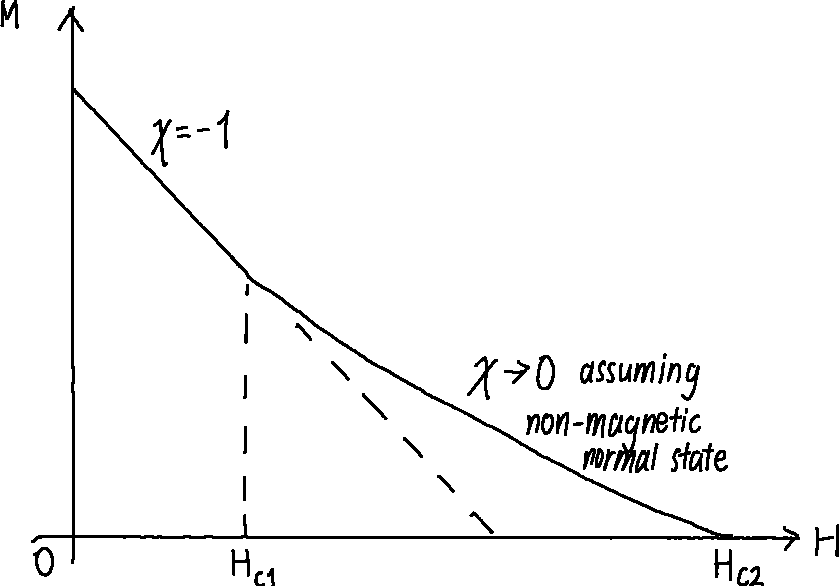
\includegraphics[width=.6\linewidth]{q5-magnetisation}
	\end{figure}
\end{parts}